Hệ thống BPSky 2.0 được triển khai giao diện thông qua Vercel với đường dẫn (url) \url{https://bpsky232.vercel.app/}. Sau khi tạo tài khoản Vercel thành công chúng ta sẽ đến với giao diện quản lý những project cá nhân. Chọn nút "Add new" để mở menu lựa chọn, chúng ta sẽ chọn "Project" để tạo mới project.

\begin{figure}[H]
    \centering
    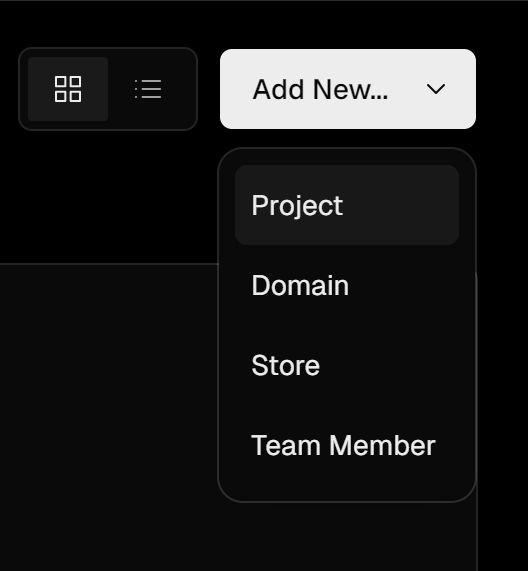
\includegraphics[width=0.3\linewidth]{Content/Hiện thực hệ thống/images/createProjectVercel.png}
    \vspace{0.5cm}
    \caption{Giao diện tạo project mới trong Vercel}
    \label{fig:Tạo project mới trong Vercel}
\end{figure}

Sau khi liên kết với tài khoản Github thì chúng ta có thể kết nối với những repository đã tạo trước đó. Chọn "Import Git Repository" và chọn repository cần triển khai. Ở đây là repository "BPE-FE-231".

\begin{figure}[H]
    \centering
    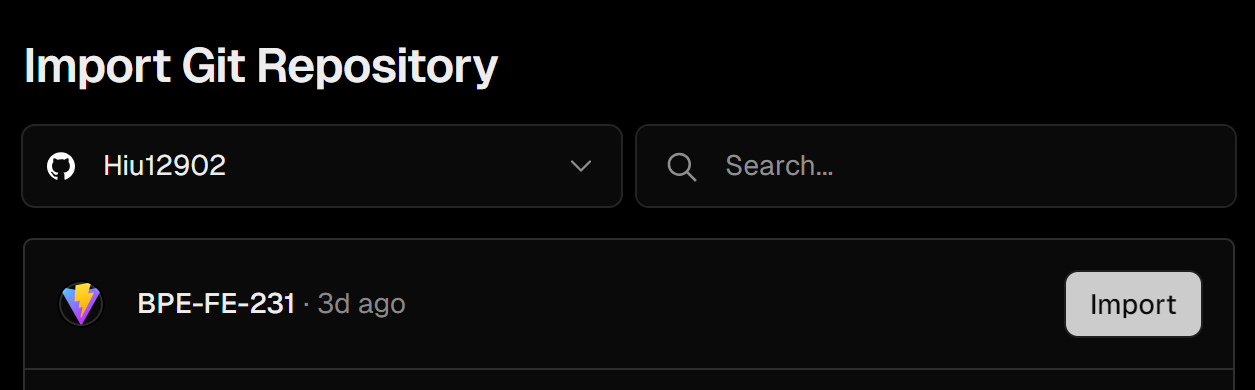
\includegraphics[width=0.5\linewidth]{Content/Hiện thực hệ thống/images/importRepoVercel.png}
    \vspace{0.5cm}
    \caption{Giao diện import repository vào Vercel}
    \label{fig:Import repository vào Vercel}
\end{figure}

Trước khi triển khai, chúng ta cần thiết lập môi trường cho project. Chọn "Environment Variables" để thêm các biến môi trường cần thiết.

\begin{figure}[H]
    \centering
    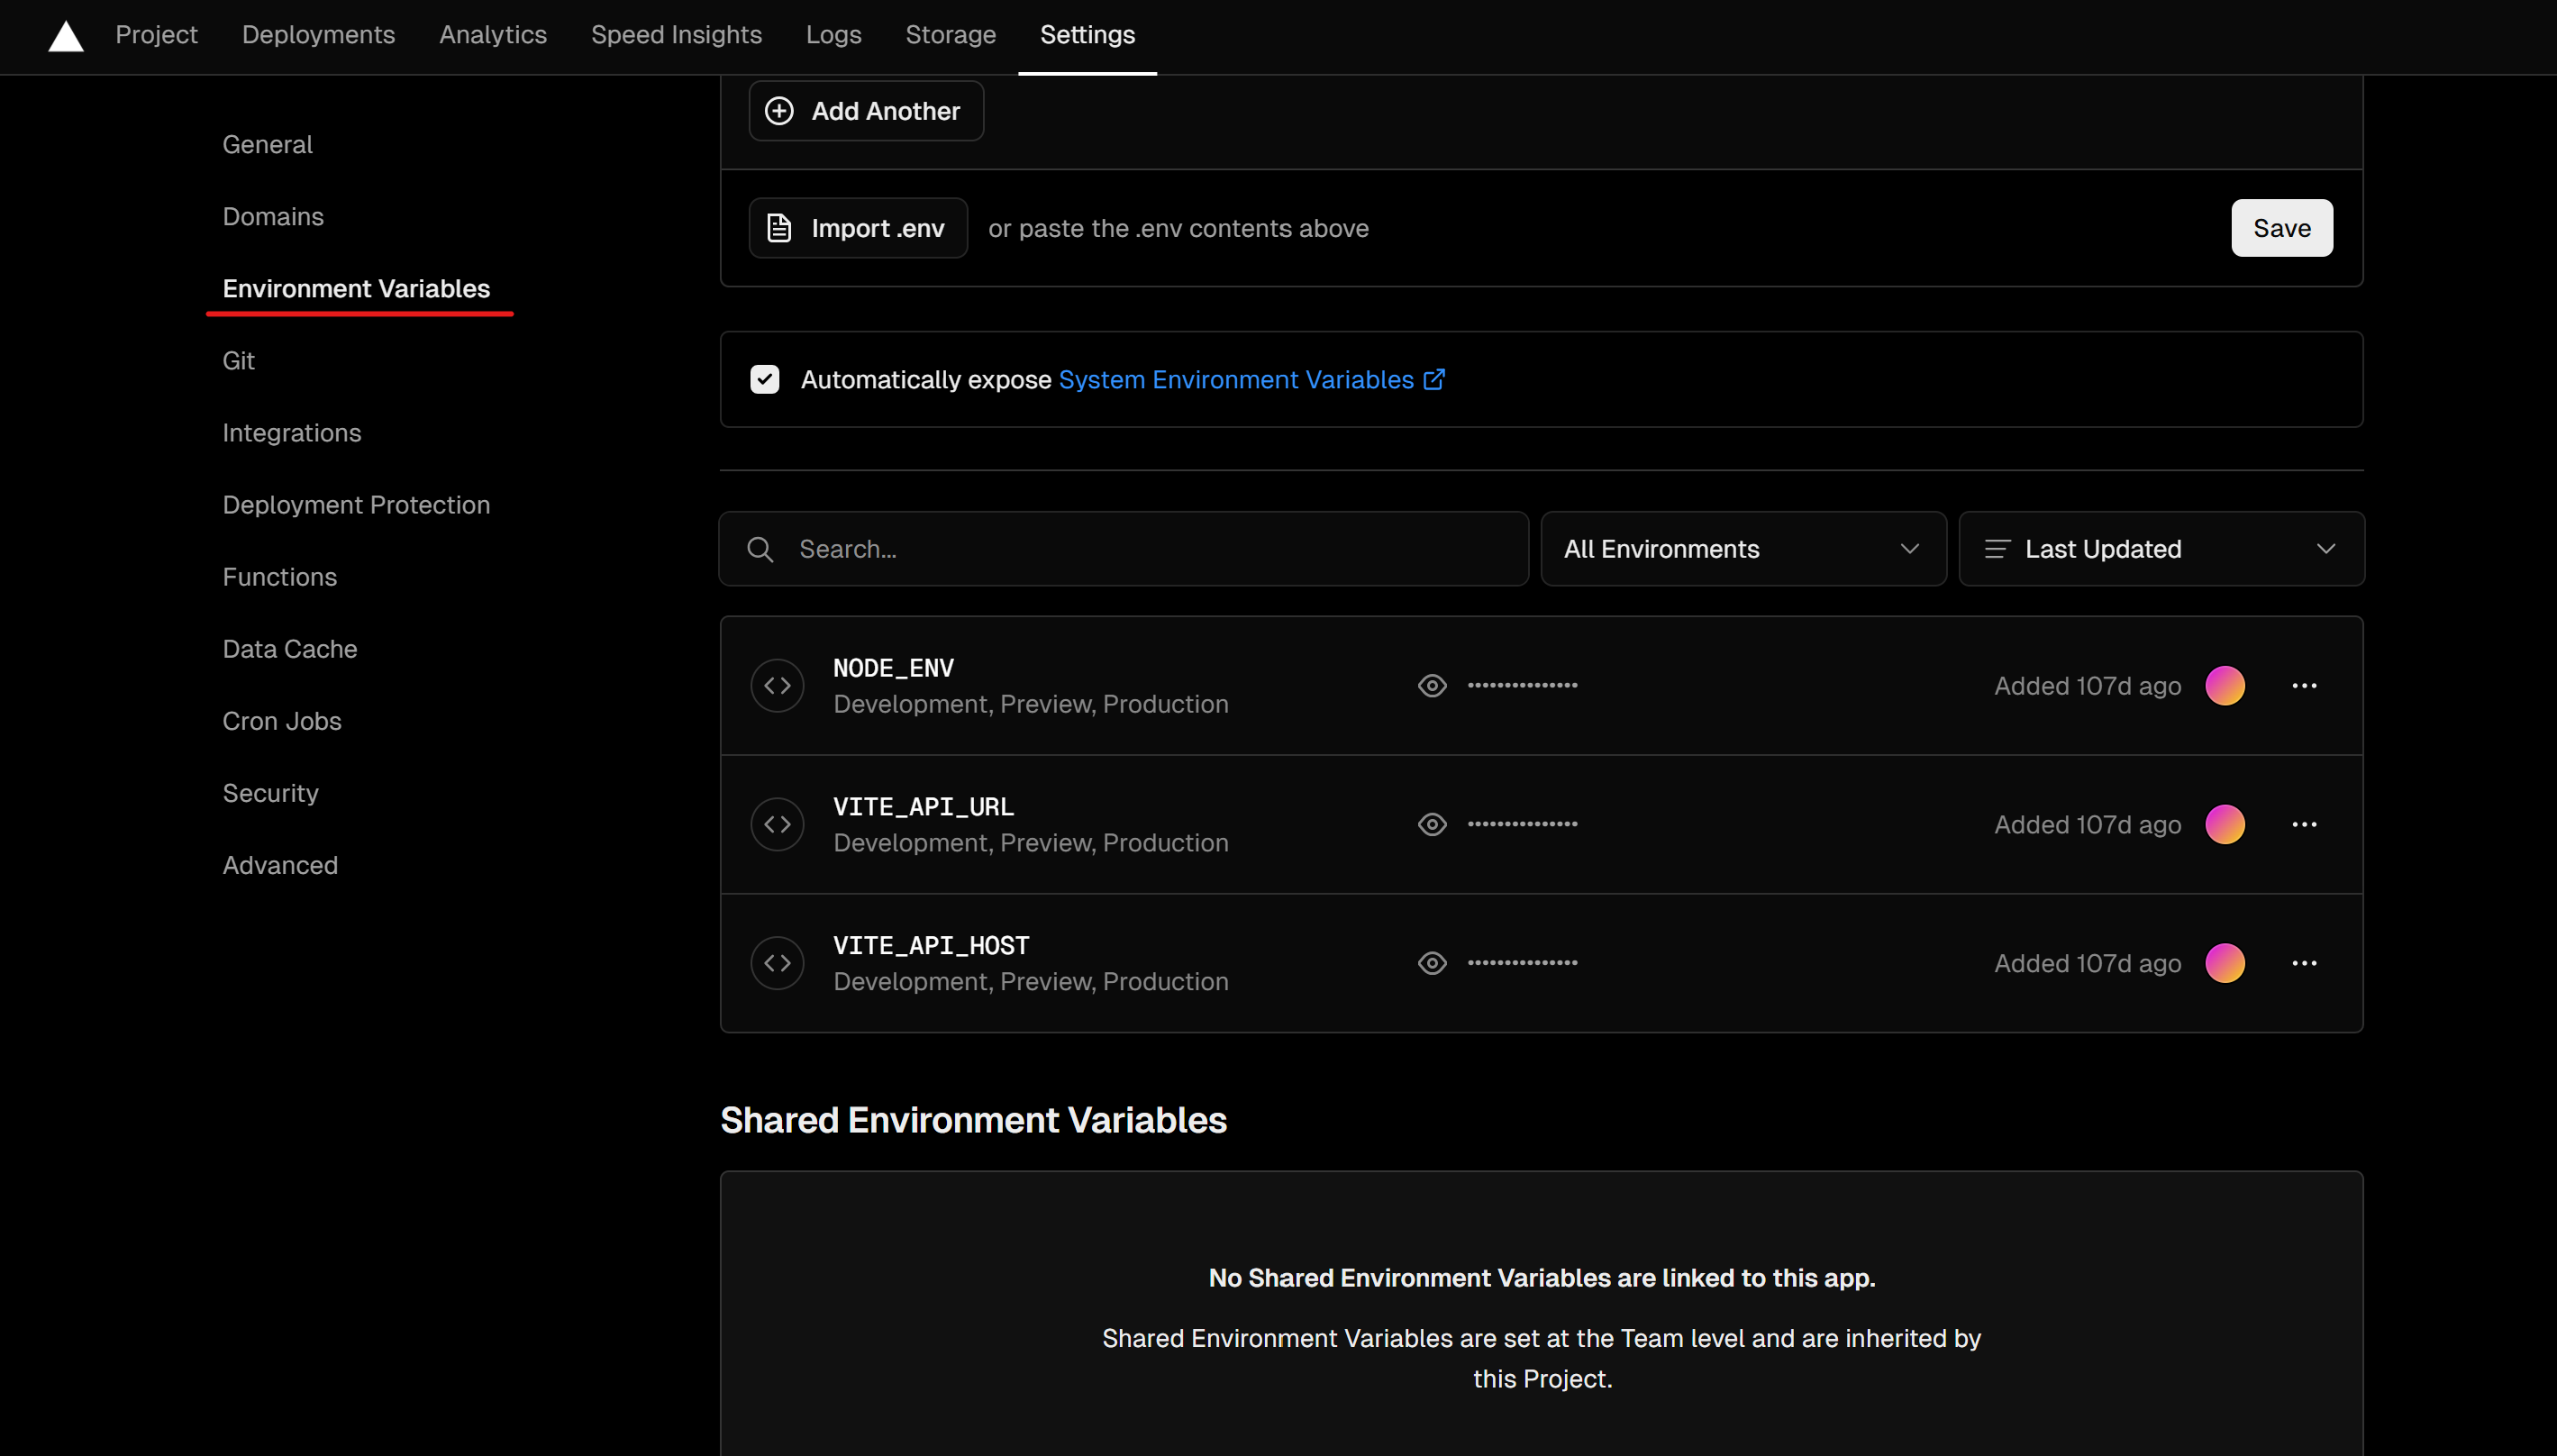
\includegraphics[width=0.7\linewidth]{Content/Hiện thực hệ thống/images/editEnvironmentVariablesVercel.png}
    \vspace{0.5cm}
    \caption{Giao diện chỉnh sửa biến môi trường trong Vercel}
    \label{fig:chỉnh sửa biến môi trường trong Vercel}
\end{figure}

Cuối cùng, chúng ta chọn "Deploy" để triển khai project. Sau khi triển khai thành công, chúng ta sẽ nhận được đường dẫn truy cập vào project. Hệ thống BPSky 2.0 được triển khai thông qua URL: https://bpsky232.vercel.app/

\begin{figure}[H]
    \centering
    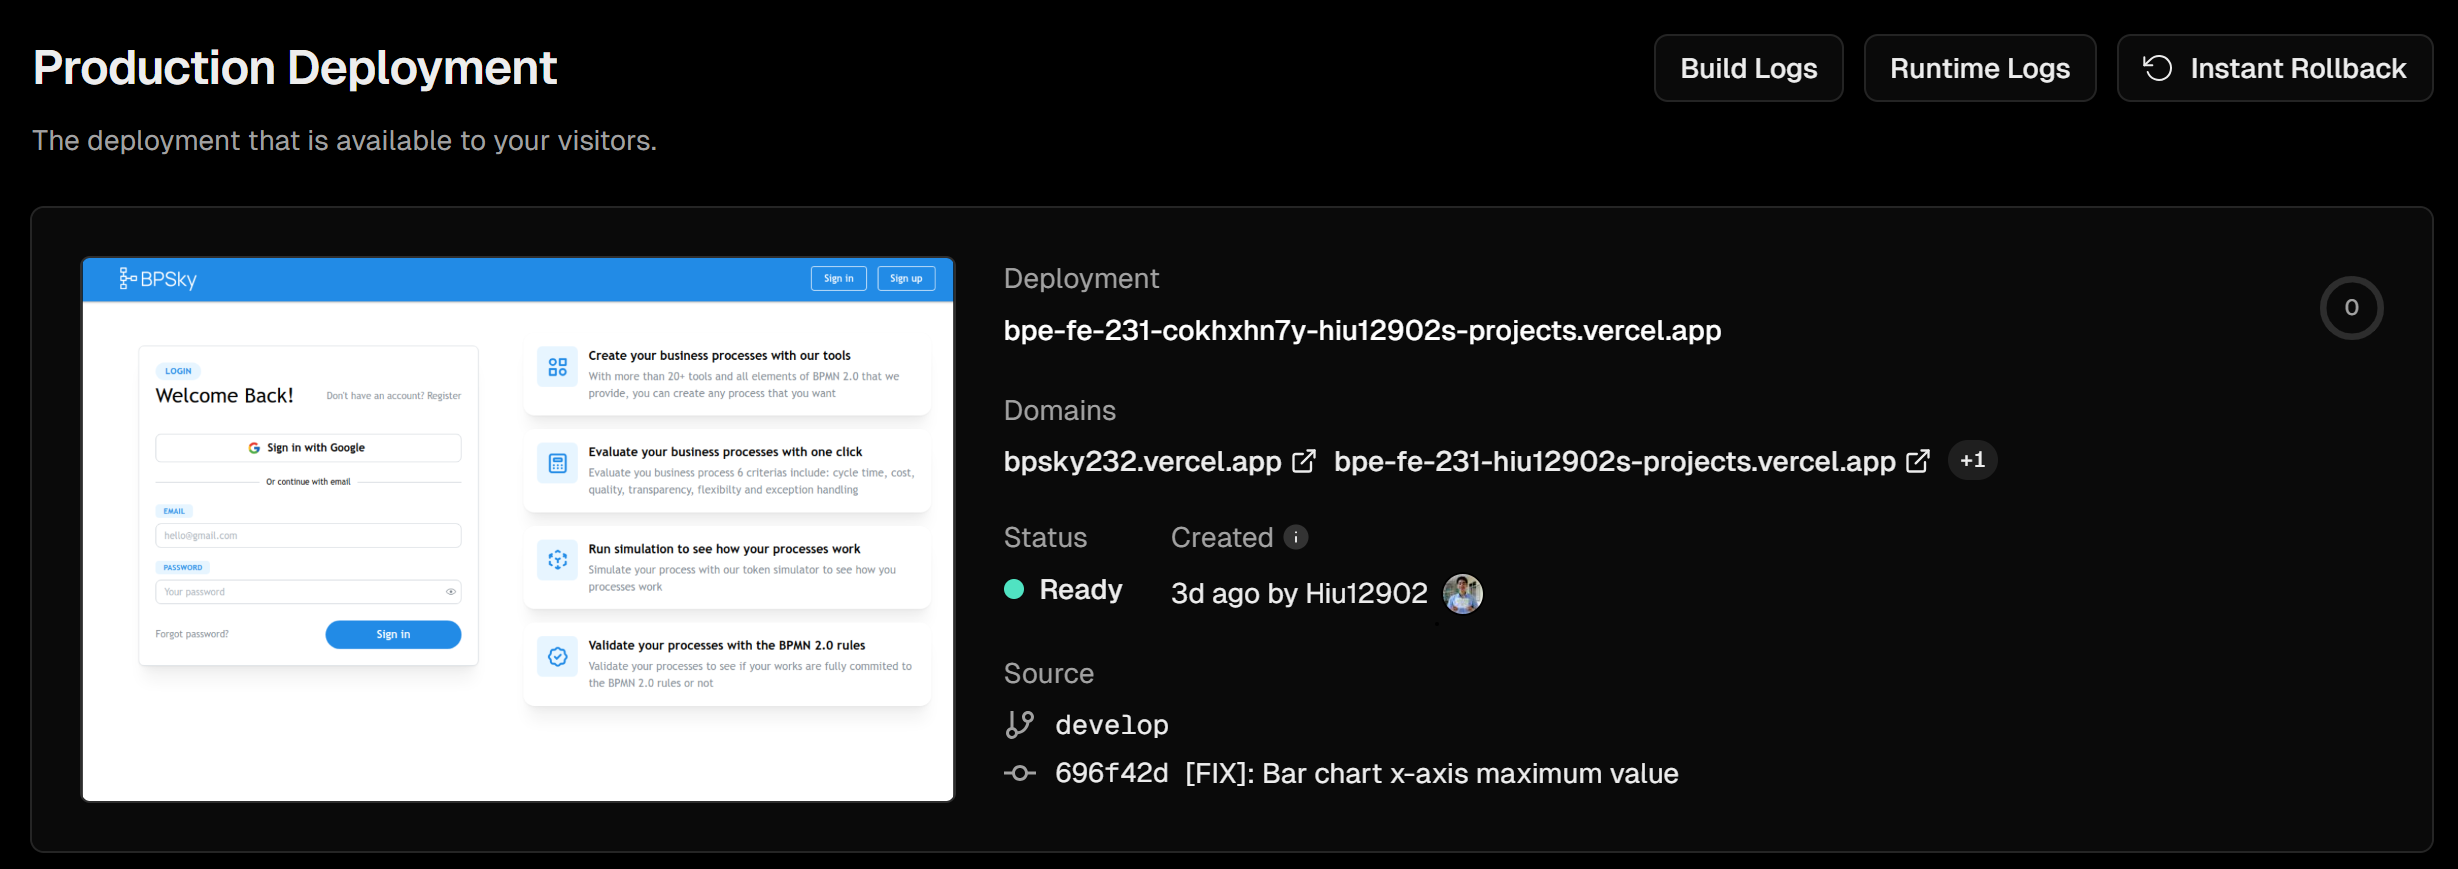
\includegraphics[width=0.7\linewidth]{Content/Hiện thực hệ thống/images/deployVercelSuccessful.png}
    \vspace{0.5cm}
    \caption{Giao diện deploy thành công trên Vercel}
    \label{fig:deploy thành công trên Vercel}
\end{figure}